<<<<<<< Updated upstream
% Compile with XeLaTeX, TeXLive 2013 or more recent
\documentclass{beamer}

% Base packages
\usepackage{fontspec}
\usepackage{xunicode}
\usepackage{xltxtra}

\usepackage{amsfonts}
\usepackage{amsmath}
\usepackage{longtable}
\usepackage{csquotes}
\usepackage{standalone}

% Setup fonts
\newfontfamily\russianfont{CMU Serif}
\setromanfont{CMU Serif}
\setsansfont{CMU Sans Serif}
\setmonofont{CMU Typewriter Text}

% Setup Russian hyphenation. NOTE: this declaration *must* come after fontspec's font declarations,
% or a mysterious (but harmless in other respects) error "Improper `at' size (0.0pt), replaced by 10pt." would appear.
\usepackage{polyglossia}
\defaultfontfeatures{Scale=MatchLowercase, Mapping=tex-text}

\setdefaultlanguage[spelling=modern]{russian} % for polyglossia
\setotherlanguage{english} % for polyglossia

% Vector drawings
\usepackage{tikz}
% \usetikzlibrary{shapes, calc, arrows, fit, positioning, decorations, patterns, decorations.pathreplacing, chains, snakes}
\usetikzlibrary{shapes, calc, arrows, decorations.markings, decorations.pathmorphing, decorations, patterns, chains, snakes, backgrounds, positioning, fit, petri}
\usepackage[siunitx]{circuitikz}

% Be able to insert hyperlinks
\usepackage{hyperref}
\hypersetup{colorlinks=true, linkcolor=black, filecolor=black, citecolor=black, urlcolor=blue , pdfauthor=Grigory Rechistov <grigory.rechistov@phystech.edu>, pdftitle=Курс «Программное моделирование вычислительных систем»}
% \usepackage{url}

% Misc optional packages
\usepackage{underscore}
\usepackage{amsthm}

% A new command to mark not done places
\newcommand{\todo}[1][Напиши меня]{{\color{red}TODO\ #1}}
\newcommand{\abbr}{\textit{англ.}\ }

\title{Моделирование центрального процессора с помощью интерпретации}
\subtitle{Курс «Программное моделирование вычислительных систем»}
\subject{Курс «Программное моделирование вычислительных систем»}

\author[]{Григорий Речистов \\ \small{\href{mailto:grigory.rechistov@phystech.edu}{grigory.rechistov@phystech.edu}}}
\date{\today}
\pgfdeclareimage[height=0.5cm]{ilab-logo}{../ilab-noletters.png}
\logo{\pgfuseimage{ilab-logo}}

\typeout{Copyright 2015 Grigory Rechistov}

\usetheme{Berlin}
\setbeamertemplate{navigation symbols}{}%remove navigation symbols

\begin{document}

\begin{frame}
    \maketitle
\end{frame}

\begin{frame}
    \tableofcontents
\end{frame}

\begin{frame}{На прошлой лекции}
Требования к симуляторам:
\begin{itemize}
\item точность,
\item скорость,
\item совместимость/расширяемость
\end{itemize}

\end{frame}

\begin{frame}{Вопросы}
\begin{itemize}
\item В чём измеряется скорость симуляции? \pause
\item Как соотносятся скорости функционального и потактового симуляторов? \pause
\item Для чего необходимо предоставлять API симулятора? \pause Чтобы пользователи могли с ним поиграть.
\end{itemize}

\end{frame}

% «»

% Use [fragile] option to insert listings
% \begin{frame}[fragile]

\section{Конвейер процессора}

\begin{frame}{Моделируемая система}
\centering
\vfill
\input{./../../simbook/metoda/drawings/cpu-mem}
\vfill
\end{frame}

\begin{frame}[shrink=0.8]{Конвейер процессора}
\centering
\input{./../../simbook/metoda/drawings/interp-cycle-expanded}
\end{frame}

\begin{frame}[fragile]{Переключаемый интерпретатор (switched)}
\begin{verbatim}
while (run) {
    raw_code = fetch(PC);
    (opcode, operands) = decode(raw_code);
    switch (opcode) {
    case opcode1:
        func1(operands); PC++; break;

    case opcode2:
        func2(operands); PC++; break;

    /*...*/
    }
}
\end{verbatim}
\end{frame}


\section{Fetch}

\begin{frame}[fragile]{Чтение инструкции из памяти}

\texttt{data = mem[pc];}\pause

Скорее,

\texttt{data = read_mem(pc);}\pause

И не забыть про преобразование адресов:

\begin{verbatim}
paddr = v2p(pc); // pc - vaddr
data = mem[paddr];
\end{verbatim}

\end{frame}

\section{Decode}

\begin{frame}{Декодирование}
Перевод данных об инструкции из машинного представления (последовательность байт) во внутреннее (высокоуровневое), удобное для последующего использования
\end{frame}

\begin{frame}{Пример: MIPS}
\centering
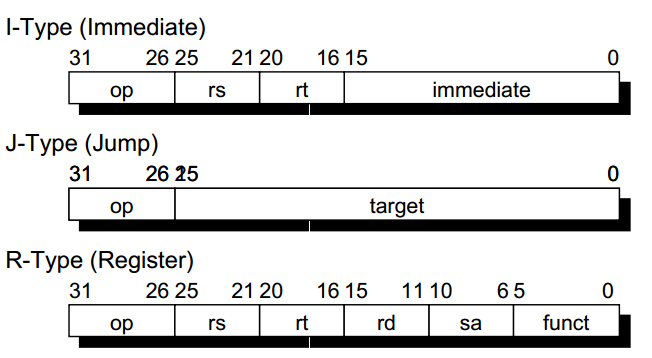
\includegraphics[width=0.8\textwidth]{./mips-formats}

\tiny{MIPS Technologies Inc. MIPS32 4K™ Processor Core Family Software User’s Manual - 2002}
\end{frame}

\begin{frame}[fragile]{Пример: код 1}
\begin{verbatim}
#define BITS(v, s, e) (v >> s) & (( 1 << (e-s+1)) - 1)

typedef struct decode {
    uint32_t op;
    uint32_t rs;
    uint32_t rt;
    int32_t  imm;
    int32_t  tgt;
    /* ... */
} decode_t;

static inline
int32_t sign_extend(uint32_t v, int width) 
    {/* ... */};
\end{verbatim}
\end{frame}

\begin{frame}[fragile]{Пример: код 2}
\begin{verbatim}
decode_t decode(uint32_t raw) {
    uint32_t op = BITS(raw, 26, 31);
    uint32_t rs = BITS(raw, 21, 25);
    uint32_t rt = BITS(raw, 16, 20);
    int32_t  imm = sign_extend(BITS(raw, 0, 15));
    int32_t  tgt = sign_extend(BITS(raw, 0, 25));
    /* ... */
    uint32_t funct = BITS(raw, 0, 5);

    return (decode_t){op, rs, rt, /* ... */, funct};
}
\end{verbatim}
\end{frame}

\begin{frame}{Более сложный пример: Intel IA-64 2.3}
\centering
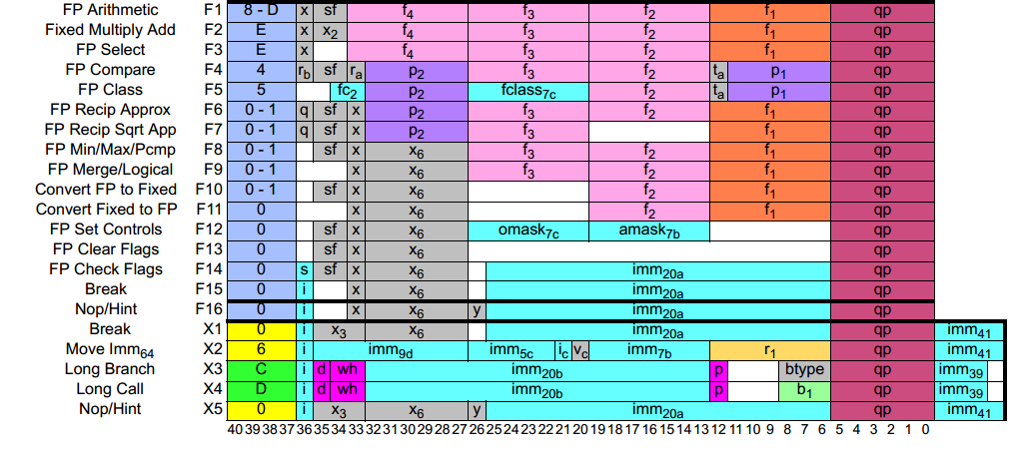
\includegraphics[width=0.95\textwidth]{./ia64-formats}

\tiny{Intel Corporation. Intel® Itanium® Architecture Software Developer’s Manual, p 3:296}

\end{frame}

\begin{frame}{Пример посложнее: Intel IA-32}
\centering
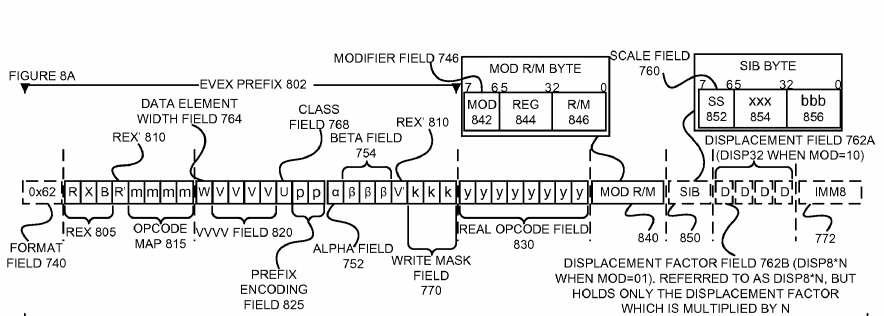
\includegraphics[width=0.95\textwidth]{./ia-32-evex}

\tiny{J.C.S. Adrian et al. Systems, Apparatuses, and Methods for Blending Two Source Operands into a Single Destination Using a Writemask. US Patent Application Publication. №~2012/0254588 A1}

\end{frame}

\begin{frame}{Что извлекать из машинного кода инструкции}
\begin{center}
% This file allows to produce either a separate PDF/PNG image
% See standalone documentation to understand underlying magic

\documentclass[tikz,convert={density=150,size=600,outext=.png}]{standalone}
\usetikzlibrary{shapes, calc, arrows, fit, positioning, decorations, patterns, decorations.pathreplacing, chains, snakes}
\input{../setup-web-fonts}
\input{../setup-packages}
\graphicspath{{../pictures/}} % path to pictures, trailing slash is mandatory.

% The actual drawing follows
\begin{document}

\tikzstyle{FatArrow} = [thick, decoration={markings,mark=at position
        1 with {\arrow[semithick]{open triangle 60}}},
        double distance=1.4pt, shorten >= 5.5pt,
        preaction = {decorate},
        postaction = {draw,line width=1.4pt, white,shorten >= 4.5pt}]

\begin{tikzpicture}[font=\footnotesize, >=latex]
    \huge
    \node[rectangle, minimum height = 0.5cm] (mnemonic) {mnemonic,};
    \node[rectangle, right = 0.5cm of mnemonic.east, minimum height = 0.5cm] (src1) {src1,};
    \node[rectangle, right = 0.5cm of src1.east, minimum height = 0.5cm] (src2) {src2,};
    \node[rectangle, right = 0.5cm of src2.east, minimum height = 0.5cm] (dst1) {dst1};
    \node[draw, rectangle, right = 1.5cm of dst1.east, minimum height = 0.5cm] (dst2) {\textcolor{gray}{dst2}};

    \node[draw, fill=green, below = 2cm of mnemonic.south, minimum height = 0.5cm] (opcode) {Код операции};
    \node[draw, below = 2cm of src2.south, minimum height = 0.5cm] (regs) {Регистры, память, константы};
    \node[draw, fill=gray, align=center, below = 1.8cm of dst2.south, minimum height = 0.5cm] (flags) {Неявные операнды:\\ флаги, PC};

    \draw[FatArrow] (mnemonic) -- (opcode);
    \draw[FatArrow] (src1) -- ([xshift = 6.5mm] regs.north west);
    \draw[FatArrow] (src2) -- (regs);
    \draw[FatArrow] (dst1) -- ([xshift = -6.7mm] regs.north east);
    \draw[FatArrow] (dst2) -- (flags);

    \draw (mnemonic.south west) -- (dst1.south east) -- (dst1.north east) -- (mnemonic.north west) -- (mnemonic.south west);
\end{tikzpicture}

\end{document}
 % TODO convert to bitfields inlines
\end{center}

На выходе декодера: 
\begin{itemize}
\item Успех, неуспех, недостаточно данных
\item Для успеха: длина инструкции
\item Для успеха: эмулирующая процедура
\end{itemize}
\end{frame}


% \begin{frame}{Декодирование}
% Задача декодирования — перевод данных об инструкции из машинного представление
% во внутреннее (высокоуровневое) удобное для последующего анализа.

% \pause

% Вход: \texttt{\textcolor{red}{0x40} \textcolor{green}{0x05} \textcolor{blue}{0xab 0x12}}

% Результат:

% \texttt{instruction \{ \\
% ~~~~opcode = \textcolor{red}{ADDI}, num\_operands = 2, \\
% ~~~~\textcolor{green}{dst = \{type = OP\_REG, reg = R5\}}, \\
% ~~~~\textcolor{blue}{src = \{type = OP\_IMM, val = 0x12ab\}}, \\
% ~~~~disasm = "addi r5, 0x12ab", \\
% ~~~~addr = 0x1234 \\
% \}}
% \end{frame}

\begin{frame}{Декодирование}
\begin{itemize}
\item Код декодера редко пишется вручную, чаще он генерируется по описанию
\item \texttt{\textcolor{red}{A5} \textcolor{blue}{Y}\textcolor{green}{X} 0\textcolor{orange}{Z} 00} $\Rightarrow$ \textcolor{red}{MOD} \textcolor{green}{RX}, \textcolor{blue}{RY}, \textcolor{orange}{RZ}
\item В общем случае: классическая задача построения  синтаксического анализатора
\item На практике: специализированные инструменты и языки
\end{itemize}
\end{frame}

\begin{frame}{Декодирование: суровая реальность}
\begin{itemize}
\item Переменная длина инструкций. IA-32: от 8 до 120 бит. Сколько байт пытаться декодировать за один раз?
\item Зависимость смысла от префикса, режима работы процессора. Пример: 0x40–0x4f в IA-32/Intel~64/AMD64
\item Полное несоответствие какому-либо здравому смыслу
\end{itemize}

\end{frame}

\begin{frame}{Дизассемблирование}
\begin{itemize}
\item Дизассемблирование — перевод инструкций из машинного представление в понятный
человеку вид (мнемонику)
\item (За)кодирование (encoding) — перевод инструкций из мнемонической записи в
машинный код
\end{itemize}
\pause
Вопрос: однозначны ли операции: декодирования, дизассемблирования, кодирования?
\end{frame}

\section{Execute}

\begin{frame}{Исполнение}

\begin{itemize}
\item Базовая единица — функция-эмулятор одной инструкции (service routine)
\item Функция-эмуляторы пишутся на языке высокого уровня $\rightarrow$ переносимость кода между хозяйскими
платформами, компиляторами

% Используются генераторы кода.

% Пример: SimGen — из одного описания генерируются декодер, дизассемблер и s.r.

\end{itemize}
\end{frame}

\begin{frame}[fragile]{Симулируемое состояние}
\begin{verbatim}
typedef struct {
    uint32_t regs[16];
    bool z_flag;
    bool n_flag;
    bool o_flag;
    bool c_flag;
    uint32_t pc;
} cpu_t;
\end{verbatim}
\end{frame}


\begin{frame}[fragile]{Пример: ADD reg reg reg}
\begin{verbatim}

void add32_rrr(cpu_t *cpu, int src1, int src2, int dst) {
    cpu->regs[dst] = cpu->regs[src1] + cpu->regs[src2];
\end{verbatim}
\pause

\begin{verbatim}
    cpu->z_flag = cpu->regs[dst] == 0;
    cpu->n_flag = cpu->regs[dst] & (1 << 31);
    cpu->o_flag = cpu->regs[dst] < 
            MAX(cpu->regs[src1], cpu->regs[src2]);
    cpu->c_flag = calc_c_flag(cpu->regs[src1],
                              cpu->regs[src2]);
}
\end{verbatim}
\end{frame}

\begin{frame}{Пример посложнее: IA-32 CALL}
\centering
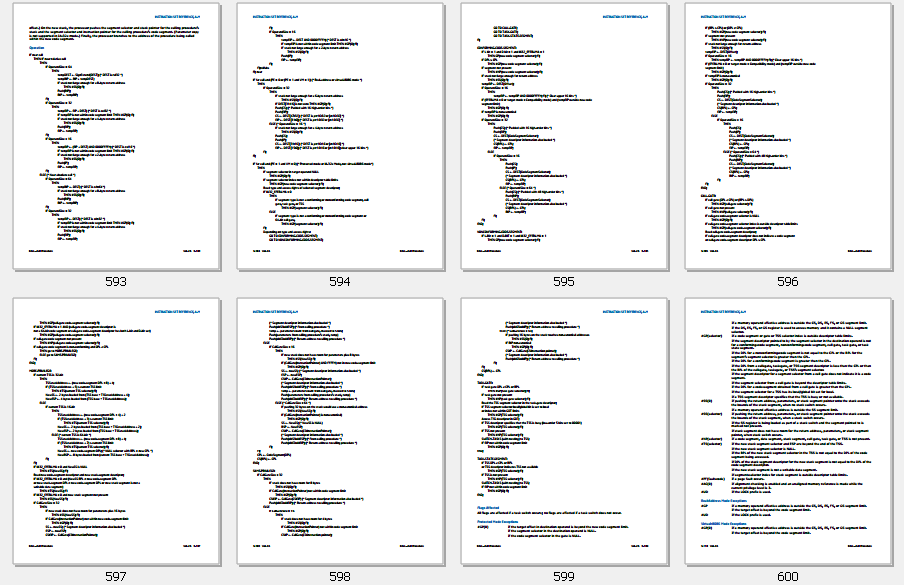
\includegraphics[width=0.95\textwidth]{./ia32-call}

\end{frame}

\section{Write Back}

\begin{frame}{Запись результата в память}
\texttt{write_mem(cpu, dst_addr, data, size);}\pause

\begin{itemize}
    \item Невыровненный адрес
    \item Граница страниц
    \item Запись в память «только для чтения»
    \item Исключения для всей или части записи/чтения
\end{itemize}

\end{frame}

\section{Исключения}

\begin{frame}[shrink=0.6]{Уточнённый цикл работы процессора}
\centering

\input{./../../simbook/metoda/drawings/interp-cycle-expanded-exception}

\end{frame}

\begin{frame}{Классификация} % TODO a tree diagram?
\begin{itemize}
\item Interruptions (термин из документации IA-64) — вмешательство, перерыв, приостановка
\item Exception — синхронное исключение, без повторения текущей инструкции
\item Fault — синхронное, с повторением текущей инструкции
\item Trap — синхронное, без повторения, намеренно вызванное
\item Interrupt — внешнее асинхронное прерывание
\item Abort — внешние асинхронное с отсутствием информации о точке возврата
\end{itemize}
\end{frame}

\section{Advance \texttt{PC}}

\begin{frame}{Продвижение \texttt{PC}}

\begin{itemize}
    \item Для большинства команд: увеличение счетчика на длину обработанной инструкции\\
    \texttt{cpu->pc += instr_length;}\\\pause
    \item Бывают исключения: \texttt{REP MOVS} в IA-32\pause
    \item Явное изменение \texttt{PC} — команды управления исполнением:
    \begin{itemize}
        \item (Без)условный (не)прямой прыжок/переход
        \item Вызов/возврат из процедуры
        \item Системный вызов
    \end{itemize}
\end{itemize}

\end{frame}

\section{Улучшенные схемы}

\begin{frame}{Преимущества и недостатки интерпретации}
\begin{itemize}
\item Пишется на языках высокого уровня: код переносим
\item Простая структура: надёжность, расширяемость, переиспользование
\end{itemize}
\pause
\begin{itemize}
\item (Очень) низкая скорость работы
\end{itemize}
\end{frame}

\begin{frame}[fragile]{Куда тратится время?}
\begin{verbatim}
start: interruption = false;
while (!interruption) {
    raw_code = fetch(PC);
    (opcode, operands) = decode(raw_code); // <-- здесь
    switch (opcode) { // <-- здесь
    case opcode1:
        func1(operands); PC++; break;
    case opcode2:
        func2(operands); PC++; break;
    /*...*/
    }
}
handle_interruption();
goto start;
\end{verbatim}
\end{frame}

\begin{frame}[fragile]{Шитая интерпретация (threaded interpretation)}
Вместо возвращения к началу цикла «прыгаем» прямо на исполнение следующей инструкции
\begin{verbatim}
func0: /* simulate instr0 */; PC++;
  next_opcode = decode(fetch(PC));
  goto func_ptr[next_opcode];
func1: /* simulate instr1 */; PC++;
  next_opcode = decode(fetch(PC));
  goto func_ptr[next_opcode];
func2: /* simulate instr2 */; PC++;
  next_opcode = decode(fetch(PC));
  goto func_ptr[next_opcode];
\end{verbatim}

\tiny\url{http://stackoverflow.com/questions/11227809/why-is-processing-a-sorted-array-faster-than-an-unsorted-array}
\end{frame}

\begin{frame}{Кэширующая интерпретация}
\begin{itemize}
\item В большинстве случаев в код гостевого приложения неизменен
\item Велика вероятность того, что инструкции с некоторыми PC будут исполнены много раз (\textit{задача})
\item Зачем каждый раз их декодировать?
\item Заводим таблицу соответствия «адрес инструкции $\rightarrow$ декодированный результат» 
\end{itemize}

\end{frame}

\begin{frame}[fragile]{Кэширующая интерпретация}
\begin{verbatim}
while (!interruption) {
  if (operation = cache[PC]); // короткий путь
  else { // не в кэше, длинный путь
  	operation = decode(fetch(PC));
  	cache[PC] = operation; // на будущее
  }
  switch (operation) {
     /* ... */
  }
}
\end{verbatim}

% 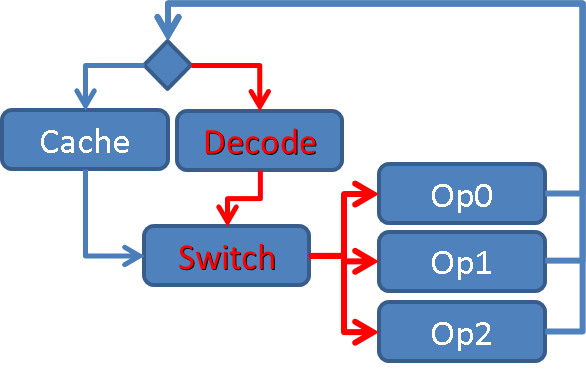
\includegraphics[width=0.3\textwidth]{./cached}

\end{frame}

\begin{frame}{Кэширующая интерпретация}
\begin{itemize}
\item Ёмкость любого кэша ограничена, старые данные надо выбрасывать
\item Необходимо следить за неизменностью исходного кода, иначе сохранённое соответствие будет неверным
\end{itemize}
\end{frame}

\begin{frame}{Итоги}
\begin{itemize}
\item Фазы исполнения: F, D, E, W, A
\item Decoder, disassembler, encoder
\item Переключаемый (switched) И.
\item Шитый (threaded) И.
\item Кэшируюший И.
\item Ситуации: interrupt, trap, exception, fault, abort
\end{itemize}
\end{frame}

\begin{frame}[allowframebreaks]{Литература}
\begin{thebibliography}{99}
    \bibitem{interpreters-comparison} Семь видов интерпретаторов виртуальной машины. В поисках самого быстрого \url{http://habrahabr.ru/company/intel/blog/261665/}
    \bibitem{bochs} D. Mihoka , S. Shwartsman. Virtualization Without Direct Execution or Jitting: Designing a Portable Virtual Machine Infrastructure \url{http://bochs.sourceforge.net/}
    \bibitem{simgen} Fredrik Larsson, Peter Magnusson, Bengt Werner. SimGen: Development of Efficient Instruction Set Simulators
\url{ftp://ftp.sics.se/pub/SICS-reports/Reports/SICS-R--97-03--SE.ps.Z}
    \bibitem{zsim} Yair Lifshitz, Robert Cohn, Inbal Livni, Omer Tabach, Mark Charney, Kim Hazelwood. Zsim: A Fast Architectural Simulator for ISA Design-Space Exploration \url{http://www.cs.virginia.edu/kim/docs/wish11zsim.pdf}
    
    \bibitem{habr1} Префиксы в системе команд IA-32 \url{http://habrahabr.ru/company/intel/blog/200598/}
    \bibitem{habr2} Программная симуляция микропроцессора. Коробка передач \url{http://habrahabr.ru/company/intel/blog/202926/}

\end{thebibliography}
\end{frame}

\begin{frame}{На следующей лекции}
Моделирование архитектурного состояния
\end{frame}


% The final "thank you" frame 
\begin{frame}

{\huge{Спасибо за внимание!}\par}

\vfill

Слайды и материалы курса доступны по адресу \url{http://is.gd/ivuboc} % http://atakua.doesntexist.org/wordpress/simulation-course-russian/

\vfill

\tiny{\textit{Замечание}: все торговые марки и логотипы, использованные в данном материале, являются собственностью их владельцев. Представленная здесь точка зрения отражает личное мнение автора, не выступающего от лица какой-либо организации.}

\end{frame}

\end{document}

/* A demo program to illustrate importance of correct branch prediction */
#include <algorithm>
#include <ctime>
#include <iostream>
int main() {
    // Generate data
    const unsigned arraySize = 32768;
    int data[arraySize];
    for (unsigned c = 0; c < arraySize; ++c)
        data[c] = std::rand() % 256;
    // Test
    clock_t start = clock();
    long long sum = 0;
    // !!! With this, the next loop runs faster
    // std::sort(data, data + arraySize);
    for (unsigned i = 0; i < 100000; ++i) {
        // Primary loop
        for (unsigned c = 0; c < arraySize; ++c) {
            if (data[c] >= 128)
                sum += data[c];
        }
    }
    double elapsedTime = static_cast<double>(clock() - start) / CLOCKS_PER_SEC;
    std::cout << elapsedTime << std::endl;
    std::cout << "sum = " << sum << std::endl;
    return 0;
}
=======
% Compile with XeLaTeX, TeXLive 2013 or more recent
\documentclass{beamer}

% Base packages
\usepackage{fontspec}
\usepackage{xunicode}
\usepackage{xltxtra}

\usepackage{amsfonts}
\usepackage{amsmath}
\usepackage{longtable}
\usepackage{csquotes}
\usepackage{standalone}

% Setup fonts
\newfontfamily\russianfont{CMU Serif}
\setromanfont{CMU Serif}
\setsansfont{CMU Sans Serif}
\setmonofont{CMU Typewriter Text}

% Setup Russian hyphenation. NOTE: this declaration *must* come after fontspec's font declarations,
% or a mysterious (but harmless in other respects) error "Improper `at' size (0.0pt), replaced by 10pt." would appear.
\usepackage{polyglossia}
\defaultfontfeatures{Scale=MatchLowercase, Mapping=tex-text}

\setdefaultlanguage[spelling=modern]{russian} % for polyglossia
\setotherlanguage{english} % for polyglossia

% Vector drawings
\usepackage{tikz}
% \usetikzlibrary{shapes, calc, arrows, fit, positioning, decorations, patterns, decorations.pathreplacing, chains, snakes}
\usetikzlibrary{shapes, calc, arrows, decorations.markings, decorations.pathmorphing, decorations, patterns, chains, snakes, backgrounds, positioning, fit, petri}
\usepackage[siunitx]{circuitikz}

% Be able to insert hyperlinks
\usepackage{hyperref}
\hypersetup{colorlinks=true, linkcolor=black, filecolor=black, citecolor=black, urlcolor=blue , pdfauthor=Grigory Rechistov <grigory.rechistov@phystech.edu>, pdftitle=Курс «Программное моделирование вычислительных систем»}
% \usepackage{url}

% Misc optional packages
\usepackage{underscore}
\usepackage{amsthm}

% A new command to mark not done places
\newcommand{\todo}[1][Напиши меня]{{\color{red}TODO\ #1}}
\newcommand{\abbr}{\textit{англ.}\ }

\title{Моделирование центрального процессора с помощью интерпретации}
\subtitle{Курс «Программное моделирование вычислительных систем»}
\subject{Курс «Программное моделирование вычислительных систем»}

\author[]{Григорий Речистов \\ \small{\href{mailto:grigory.rechistov@phystech.edu}{grigory.rechistov@phystech.edu}}}
\date{\today}
\pgfdeclareimage[height=0.5cm]{ilab-logo}{../ilab-noletters.png}
\logo{\pgfuseimage{ilab-logo}}

\typeout{Copyright 2015 Grigory Rechistov}

\usetheme{Berlin}
\setbeamertemplate{navigation symbols}{}%remove navigation symbols

\begin{document}

\begin{frame}
    \maketitle
\end{frame}

\begin{frame}
    \tableofcontents
\end{frame}

\begin{frame}{На прошлой лекции}
Требования к симуляторам:
\begin{itemize}
\item точность,
\item скорость,
\item совместимость/расширяемость
\end{itemize}

\end{frame}

\begin{frame}{Вопросы}
\begin{itemize}
\item В чём измеряется скорость симуляции? \pause
\item Как соотносятся скорости функционального и потактового симуляторов? \pause
\item Для чего необходимо предоставлять API симулятора? \pause Чтобы пользователи могли с ним поиграть.
\end{itemize}

\end{frame}

% «»

% Use [fragile] option to insert listings
% \begin{frame}[fragile]

\section{Конвейер процессора}

\begin{frame}{Моделируемая система}
\centering
\vfill
\input{./../../simbook/metoda/drawings/cpu-mem}
\vfill
\end{frame}

\begin{frame}[shrink=0.8]{Конвейер процессора}
\centering
\input{./../../simbook/metoda/drawings/interp-cycle-expanded}
\end{frame}

\begin{frame}[fragile]{Переключаемый интерпретатор (switched)}
\begin{verbatim}
while (run) {
    raw_code = fetch(PC);
    (opcode, operands) = decode(raw_code);
    switch (opcode) {
    case opcode1:
        func1(operands); PC++; break;

    case opcode2:
        func2(operands); PC++; break;

    /*...*/
    }
}
\end{verbatim}
\end{frame}


\section{Fetch}

\begin{frame}[fragile]{Чтение инструкции из памяти}

\texttt{data = mem[pc];}\pause

Скорее,

\texttt{data = read_mem(pc);}\pause

И не забыть про преобразование адресов:

\begin{verbatim}
paddr = v2p(pc); // pc - vaddr
data = mem[paddr];
\end{verbatim}

\end{frame}

\section{Decode}

\begin{frame}{Декодирование}
Перевод данных об инструкции из машинного представления (последовательность байт) во внутреннее (высокоуровневое), удобное для последующего использования
\end{frame}

\begin{frame}{Пример: MIPS}
\centering
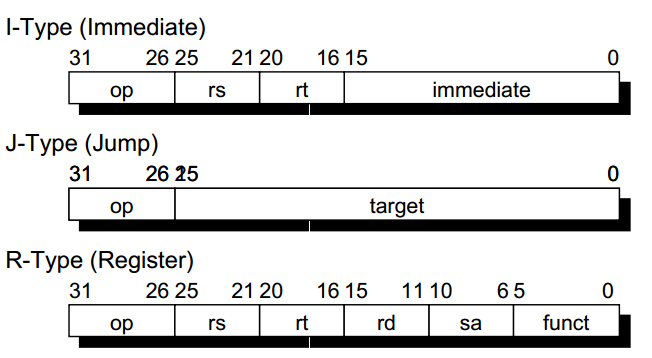
\includegraphics[width=0.8\textwidth]{./mips-formats}

\tiny{MIPS Technologies Inc. MIPS32 4K™ Processor Core Family Software User’s Manual - 2002}
\end{frame}

\begin{frame}[fragile]{Пример: код 1}
\begin{verbatim}
#define BITS(v, s, e) (v >> s) & (( 1 << (e-s+1)) - 1)

typedef struct decode {
    uint32_t op;
    uint32_t rs;
    uint32_t rt;
    int32_t  imm;
    int32_t  tgt;
    /* ... */
} decode_t;

static inline
int32_t sign_extend(uint32_t v, int width) 
    {/* ... */};
\end{verbatim}
\end{frame}

\begin{frame}[fragile]{Пример: код 2}
\begin{verbatim}
decode_t decode(uint32_t raw) {
    uint32_t op = BITS(raw, 26, 31);
    uint32_t rs = BITS(raw, 21, 25);
    uint32_t rt = BITS(raw, 16, 20);
    int32_t  imm = sign_extend(BITS(raw, 0, 15));
    int32_t  tgt = sign_extend(BITS(raw, 0, 25));
    /* ... */
    uint32_t funct = BITS(raw, 0, 5);

    return (decode_t){op, rs, rt, /* ... */, funct};
}
\end{verbatim}
\end{frame}

\begin{frame}{Более сложный пример: Intel IA-64 2.3}
\centering
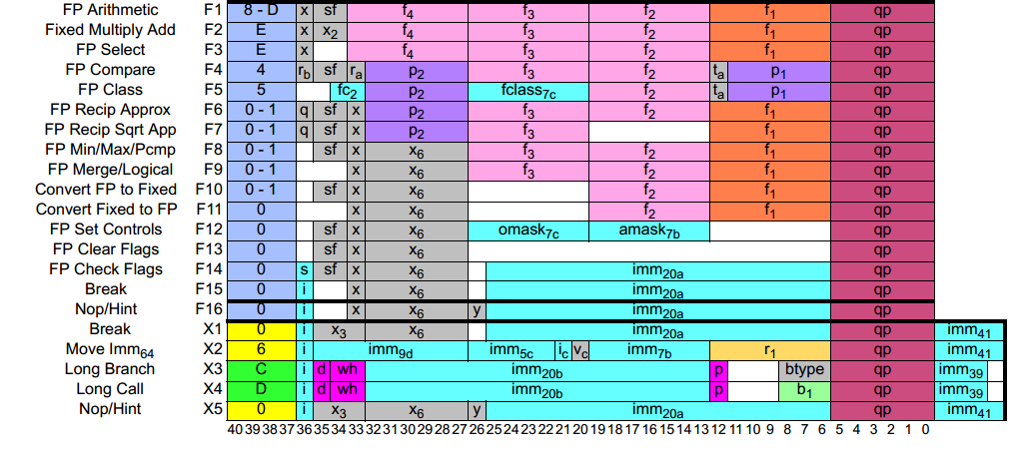
\includegraphics[width=0.95\textwidth]{./ia64-formats}

\tiny{Intel Corporation. Intel® Itanium® Architecture Software Developer’s Manual, p 3:296}

\end{frame}

\begin{frame}{Пример посложнее: Intel IA-32}
\centering
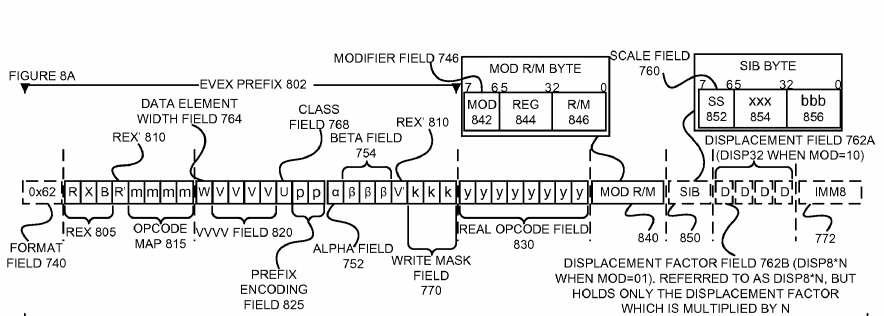
\includegraphics[width=0.95\textwidth]{./ia-32-evex}

\tiny{J.C.S. Adrian et al. Systems, Apparatuses, and Methods for Blending Two Source Operands into a Single Destination Using a Writemask. US Patent Application Publication. №~2012/0254588 A1}

\end{frame}

\begin{frame}{Что извлекать из машинного кода инструкции}
\begin{center}
% This file allows to produce either a separate PDF/PNG image
% See standalone documentation to understand underlying magic

\documentclass[tikz,convert={density=150,size=600,outext=.png}]{standalone}
\usetikzlibrary{shapes, calc, arrows, fit, positioning, decorations, patterns, decorations.pathreplacing, chains, snakes}
\input{../setup-web-fonts}
\input{../setup-packages}
\graphicspath{{../pictures/}} % path to pictures, trailing slash is mandatory.

% The actual drawing follows
\begin{document}

\tikzstyle{FatArrow} = [thick, decoration={markings,mark=at position
        1 with {\arrow[semithick]{open triangle 60}}},
        double distance=1.4pt, shorten >= 5.5pt,
        preaction = {decorate},
        postaction = {draw,line width=1.4pt, white,shorten >= 4.5pt}]

\begin{tikzpicture}[font=\footnotesize, >=latex]
    \huge
    \node[rectangle, minimum height = 0.5cm] (mnemonic) {mnemonic,};
    \node[rectangle, right = 0.5cm of mnemonic.east, minimum height = 0.5cm] (src1) {src1,};
    \node[rectangle, right = 0.5cm of src1.east, minimum height = 0.5cm] (src2) {src2,};
    \node[rectangle, right = 0.5cm of src2.east, minimum height = 0.5cm] (dst1) {dst1};
    \node[draw, rectangle, right = 1.5cm of dst1.east, minimum height = 0.5cm] (dst2) {\textcolor{gray}{dst2}};

    \node[draw, fill=green, below = 2cm of mnemonic.south, minimum height = 0.5cm] (opcode) {Код операции};
    \node[draw, below = 2cm of src2.south, minimum height = 0.5cm] (regs) {Регистры, память, константы};
    \node[draw, fill=gray, align=center, below = 1.8cm of dst2.south, minimum height = 0.5cm] (flags) {Неявные операнды:\\ флаги, PC};

    \draw[FatArrow] (mnemonic) -- (opcode);
    \draw[FatArrow] (src1) -- ([xshift = 6.5mm] regs.north west);
    \draw[FatArrow] (src2) -- (regs);
    \draw[FatArrow] (dst1) -- ([xshift = -6.7mm] regs.north east);
    \draw[FatArrow] (dst2) -- (flags);

    \draw (mnemonic.south west) -- (dst1.south east) -- (dst1.north east) -- (mnemonic.north west) -- (mnemonic.south west);
\end{tikzpicture}

\end{document}
 % TODO convert to bitfields inlines
\end{center}

На выходе декодера: 
\begin{itemize}
\item Успех, неуспех, недостаточно данных
\item Для успеха: длина инструкции
\item Для успеха: эмулирующая процедура
\end{itemize}
\end{frame}


% \begin{frame}{Декодирование}
% Задача декодирования — перевод данных об инструкции из машинного представление
% во внутреннее (высокоуровневое) удобное для последующего анализа.

% \pause

% Вход: \texttt{\textcolor{red}{0x40} \textcolor{green}{0x05} \textcolor{blue}{0xab 0x12}}

% Результат:

% \texttt{instruction \{ \\
% ~~~~opcode = \textcolor{red}{ADDI}, num\_operands = 2, \\
% ~~~~\textcolor{green}{dst = \{type = OP\_REG, reg = R5\}}, \\
% ~~~~\textcolor{blue}{src = \{type = OP\_IMM, val = 0x12ab\}}, \\
% ~~~~disasm = "addi r5, 0x12ab", \\
% ~~~~addr = 0x1234 \\
% \}}
% \end{frame}

\begin{frame}{Декодирование}
\begin{itemize}
\item Код декодера редко пишется вручную, чаще он генерируется по описанию
\item \texttt{\textcolor{red}{A5} \textcolor{blue}{Y}\textcolor{green}{X} 0\textcolor{orange}{Z} 00} $\Rightarrow$ \textcolor{red}{MOD} \textcolor{green}{RX}, \textcolor{blue}{RY}, \textcolor{orange}{RZ}
\item В общем случае: классическая задача построения  синтаксического анализатора
\item На практике: специализированные инструменты и языки
\end{itemize}
\end{frame}

\begin{frame}{Декодирование: суровая реальность}
\begin{itemize}
\item Переменная длина инструкций. IA-32: от 8 до 120 бит. Сколько байт пытаться декодировать за один раз?
\item Зависимость смысла от префикса, режима работы процессора. Пример: 0x40–0x4f в IA-32/Intel~64/AMD64
\item Полное несоответствие какому-либо здравому смыслу
\end{itemize}

\end{frame}

\begin{frame}{Дизассемблирование}
\begin{itemize}
\item Дизассемблирование — перевод инструкций из машинного представление в понятный
человеку вид (мнемонику)
\item (За)кодирование (encoding) — перевод инструкций из мнемонической записи в
машинный код
\end{itemize}
\pause
Вопрос: однозначны ли операции: декодирования, дизассемблирования, кодирования?
\end{frame}

\section{Execute}

\begin{frame}{Исполнение}

\begin{itemize}
\item Базовая единица — функция-эмулятор одной инструкции (service routine)
\item Функция-эмуляторы пишутся на языке высокого уровня $\rightarrow$ переносимость кода между хозяйскими
платформами, компиляторами

% Используются генераторы кода.

% Пример: SimGen — из одного описания генерируются декодер, дизассемблер и s.r.

\end{itemize}
\end{frame}

\begin{frame}[fragile]{Симулируемое состояние}
\begin{verbatim}
typedef struct {
    uint32_t regs[16];
    bool z_flag;
    bool n_flag;
    bool o_flag;
    bool c_flag;
    uint32_t pc;
} cpu_t;
\end{verbatim}
\end{frame}


\begin{frame}[fragile]{Пример: ADD reg reg reg}
\begin{verbatim}

void add32_rrr(cpu_t *cpu, int src1, int src2, int dst) {
    cpu->regs[dst] = cpu->regs[src1] + cpu->regs[src2];
\end{verbatim}
\pause

\begin{verbatim}
    cpu->z_flag = cpu->regs[dst] == 0;
    cpu->n_flag = cpu->regs[dst] & (1 << 31);
    cpu->o_flag = cpu->regs[dst] < 
            MAX(cpu->regs[src1], cpu->regs[src2]);
    cpu->c_flag = calc_c_flag(cpu->regs[src1],
                              cpu->regs[src2]);
}
\end{verbatim}
\end{frame}

\begin{frame}{Пример посложнее: IA-32 CALL}
\centering
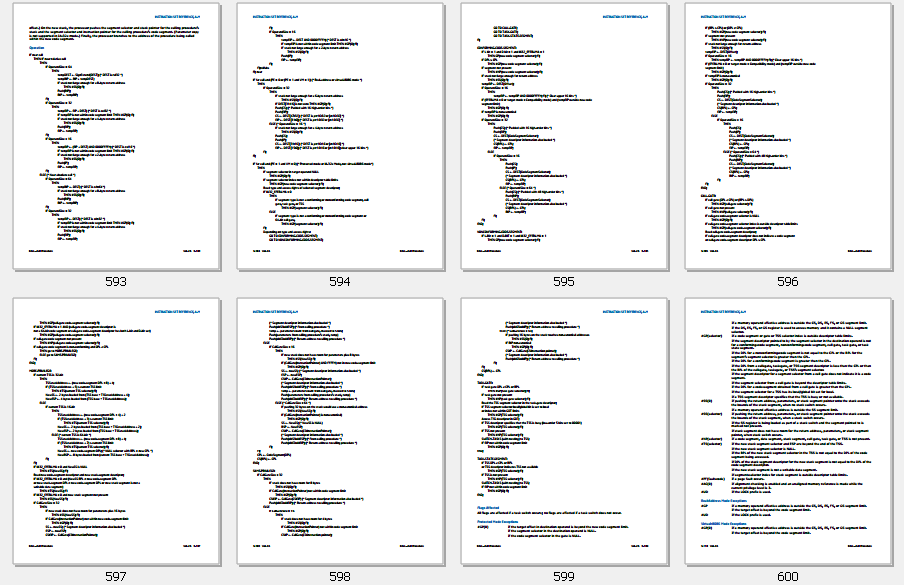
\includegraphics[width=0.95\textwidth]{./ia32-call}

\end{frame}

\section{Write Back}

\begin{frame}{Запись результата в память}
\texttt{write_mem(cpu, dst_addr, data, size);}\pause

\begin{itemize}
    \item Невыровненный адрес
    \item Граница страниц
    \item Запись в память «только для чтения»
    \item Исключения для всей или части записи/чтения
\end{itemize}

\end{frame}

\section{Исключения}

\begin{frame}[shrink=0.6]{Уточнённый цикл работы процессора}
\centering

\input{./../../simbook/metoda/drawings/interp-cycle-expanded-exception}

\end{frame}

\begin{frame}{Классификация} % TODO a tree diagram?
\begin{itemize}
\item Interruptions (термин из документации IA-64) — вмешательство, перерыв, приостановка
\item Exception — синхронное исключение, без повторения текущей инструкции
\item Fault — синхронное, с повторением текущей инструкции
\item Trap — синхронное, без повторения, намеренно вызванное
\item Interrupt — внешнее асинхронное прерывание
\item Abort — внешние асинхронное с отсутствием информации о точке возврата
\end{itemize}
\end{frame}

\section{Advance \texttt{PC}}

\begin{frame}{Продвижение \texttt{PC}}

\begin{itemize}
    \item Для большинства команд: увеличение счетчика на длину обработанной инструкции\\
    \texttt{cpu->pc += instr_length;}\\\pause
    \item Бывают исключения: \texttt{REP MOVS} в IA-32\pause
    \item Явное изменение \texttt{PC} — команды управления исполнением:
    \begin{itemize}
        \item (Без)условный (не)прямой прыжок/переход
        \item Вызов/возврат из процедуры
        \item Системный вызов
    \end{itemize}
\end{itemize}

\end{frame}

\section{Улучшенные схемы}

\begin{frame}{Преимущества и недостатки интерпретации}
\begin{itemize}
\item Пишется на языках высокого уровня: код переносим
\item Простая структура: надёжность, расширяемость, переиспользование
\end{itemize}
\pause
\begin{itemize}
\item (Очень) низкая скорость работы
\end{itemize}
\end{frame}

\begin{frame}[fragile]{Куда тратится время?}
\begin{verbatim}
start: interruption = false;
while (!interruption) {
    raw_code = fetch(PC);
    (opcode, operands) = decode(raw_code); // <-- здесь
    switch (opcode) { // <-- здесь
    case opcode1:
        func1(operands); PC++; break;
    case opcode2:
        func2(operands); PC++; break;
    /*...*/
    }
}
handle_interruption();
goto start;
\end{verbatim}
\end{frame}

\begin{frame}[fragile]{Шитая интерпретация (threaded interpretation)}
Вместо возвращения к началу цикла «прыгаем» прямо на исполнение следующей инструкции
\begin{verbatim}
func0: /* simulate instr0 */; PC++;
  next_opcode = decode(fetch(PC));
  goto func_ptr[next_opcode];
func1: /* simulate instr1 */; PC++;
  next_opcode = decode(fetch(PC));
  goto func_ptr[next_opcode];
func2: /* simulate instr2 */; PC++;
  next_opcode = decode(fetch(PC));
  goto func_ptr[next_opcode];
\end{verbatim}

\tiny\url{http://stackoverflow.com/questions/11227809/why-is-processing-a-sorted-array-faster-than-an-unsorted-array}
\end{frame}

\begin{frame}{Кэширующая интерпретация}
\begin{itemize}
\item В большинстве случаев в код гостевого приложения неизменен
\item Велика вероятность того, что инструкции с некоторыми PC будут исполнены много раз (\textit{задача})
\item Зачем каждый раз их декодировать?
\item Заводим таблицу соответствия «адрес инструкции $\rightarrow$ декодированный результат» 
\end{itemize}

\end{frame}

\begin{frame}[fragile]{Кэширующая интерпретация}
\begin{verbatim}
while (!interruption) {
  if (operation = cache[PC]); // короткий путь
  else { // не в кэше, длинный путь
  	operation = decode(fetch(PC));
  	cache[PC] = operation; // на будущее
  }
  switch (operation) {
     /* ... */
  }
}
\end{verbatim}

% 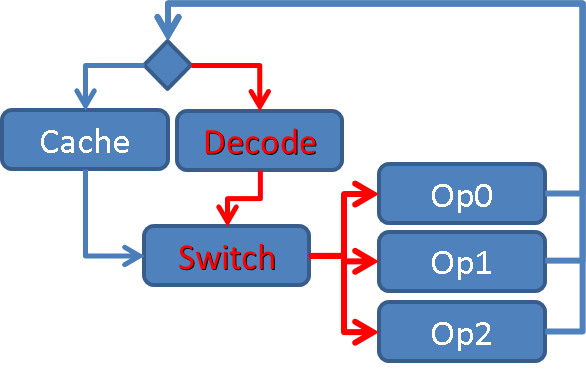
\includegraphics[width=0.3\textwidth]{./cached}

\end{frame}

\begin{frame}{Кэширующая интерпретация}
\begin{itemize}
\item Ёмкость любого кэша ограничена, старые данные надо выбрасывать
\item Необходимо следить за неизменностью исходного кода, иначе сохранённое соответствие будет неверным
\end{itemize}
\end{frame}

\begin{frame}{Итоги}
\begin{itemize}
\item Фазы исполнения: F, D, E, W, A
\item Decoder, disassembler, encoder
\item Переключаемый (switched) И.
\item Шитый (threaded) И.
\item Кэшируюший И.
\item Ситуации: interrupt, trap, exception, fault, abort
\end{itemize}
\end{frame}

\begin{frame}[allowframebreaks]{Литература}
\begin{thebibliography}{99}
    \bibitem{bochs} D. Mihoka , S. Shwartsman. Virtualization Without Direct Execution or Jitting: Designing a Portable Virtual Machine Infrastructure \url{http://bochs.sourceforge.net/}
    \bibitem{simgen} Fredrik Larsson, Peter Magnusson, Bengt Werner. SimGen: Development of Efficient Instruction Set Simulators
\url{ftp://ftp.sics.se/pub/SICS-reports/Reports/SICS-R--97-03--SE.ps.Z}
    \bibitem{zsim} Yair Lifshitz, Robert Cohn, Inbal Livni, Omer Tabach, Mark Charney, Kim Hazelwood. Zsim: A Fast Architectural Simulator for ISA Design-Space Exploration \url{http://www.cs.virginia.edu/kim/docs/wish11zsim.pdf}
    
    \bibitem{habr1} Префиксы в системе команд IA-32 \url{http://habrahabr.ru/company/intel/blog/200598/}
    \bibitem{habr2} Программная симуляция микропроцессора. Коробка передач \url{http://habrahabr.ru/company/intel/blog/202926/}

\end{thebibliography}
\end{frame}

\begin{frame}{На следующей лекции}
Моделирование архитектурного состояния
\end{frame}


% The final "thank you" frame 
\begin{frame}

{\huge{Спасибо за внимание!}\par}

\vfill

Слайды и материалы курса доступны по адресу \url{http://is.gd/ivuboc} % http://atakua.doesntexist.org/wordpress/simulation-course-russian/

\vfill

\tiny{\textit{Замечание}: все торговые марки и логотипы, использованные в данном материале, являются собственностью их владельцев. Представленная здесь точка зрения отражает личное мнение автора, не выступающего от лица какой-либо организации.}

\end{frame}

\end{document}

/* A demo program to illustrate importance of correct branch prediction */
#include <algorithm>
#include <ctime>
#include <iostream>
int main() {
    // Generate data
    const unsigned arraySize = 32768;
    int data[arraySize];
    for (unsigned c = 0; c < arraySize; ++c)
        data[c] = std::rand() % 256;
    // Test
    clock_t start = clock();
    long long sum = 0;
    // !!! With this, the next loop runs faster
    // std::sort(data, data + arraySize);
    for (unsigned i = 0; i < 100000; ++i) {
        // Primary loop
        for (unsigned c = 0; c < arraySize; ++c) {
            if (data[c] >= 128)
                sum += data[c];
        }
    }
    double elapsedTime = static_cast<double>(clock() - start) / CLOCKS_PER_SEC;
    std::cout << elapsedTime << std::endl;
    std::cout << "sum = " << sum << std::endl;
    return 0;
}
>>>>>>> Stashed changes
